%% bare_jrnl_transmag.tex
%% V1.4
%% 2012/12/27
%% by Michael Shell
%% see http://www.michaelshell.org/
%% for current contact information.
%%
%% This is a skeleton file demonstrating the use of IEEEtran.cls
%% (requires IEEEtran.cls version 1.8 or later) with an IEEE 
%% Transactions on Magnetics journal paper.
%%
%% Support sites:
%% http://www.michaelshell.org/tex/ieeetran/
%% http://www.ctan.org/tex-archive/macros/latex/contrib/IEEEtran/
%% and
%% http://www.ieee.org/



% *** Authors should verify (and, if needed, correct) their LaTeX system  ***
% *** with the testflow diagnostic prior to trusting their LaTeX platform ***
% *** with production work. IEEE's font choices can trigger bugs that do  ***
% *** not appear when using other class files.                            ***
% The testflow support page is at:
% http://www.michaelshell.org/tex/testflow/


%%*************************************************************************
%% Legal Notice:
%% This code is offered as-is without any warranty either expressed or
%% implied; without even the implied warranty of MERCHANTABILITY or
%% FITNESS FOR A PARTICULAR PURPOSE! 
%% User assumes all risk.
%% In no event shall IEEE or any contributor to this code be liable for
%% any damages or losses, including, but not limited to, incidental,
%% consequential, or any other damages, resulting from the use or misuse
%% of any information contained here.
%%
%% All comments are the opinions of their respective authors and are not
%% necessarily endorsed by the IEEE.
%%
%% This work is distributed under the LaTeX Project Public License (LPPL)
%% ( http://www.latex-project.org/ ) version 1.3, and may be freely used,
%% distributed and modified. A copy of the LPPL, version 1.3, is included
%% in the base LaTeX documentation of all distributions of LaTeX released
%% 2003/12/01 or later.
%% Retain all contribution notices and credits.
%% ** Modified files should be clearly indicated as such, including  **
%% ** renaming them and changing author support contact information. **
%%
%% File list of work: IEEEtran.cls, IEEEtran_HOWTO.pdf, bare_adv.tex,
%%                    bare_conf.tex, bare_jrnl.tex, bare_jrnl_compsoc.tex,
%%                    bare_jrnl_transmag.tex
%%*************************************************************************

% Note that the a4paper option is mainly intended so that authors in
% countries using A4 can easily print to A4 and see how their papers will
% look in print - the typesetting of the document will not typically be
% affected with changes in paper size (but the bottom and side margins will).
% Use the testflow package mentioned above to verify correct handling of
% both paper sizes by the user's LaTeX system.
%
% Also note that the "draftcls" or "draftclsnofoot", not "draft", option
% should be used if it is desired that the figures are to be displayed in
% draft mode.
%

\documentclass[journal,trans]{IEEEtran}

\usepackage[utf8]{inputenc}
\usepackage{graphicx}
\usepackage[es-tabla,spanish,activeacute]{babel}
\usepackage{amsmath}
\usepackage{breqn}
%
% If IEEEtran.cls has not been installed into the LaTeX system files,
% manually specify the path to it like:
% \documentclass[journal]{../sty/IEEEtran}





% Some very useful LaTeX packages include:
% (uncomment the ones you want to load)


% *** MISC UTILITY PACKAGES ***
%
%\usepackage{ifpdf}
% Heiko Oberdiek's ifpdf.sty is very useful if you need conditional
% compilation based on whether the output is pdf or dvi.
% usage:
% \ifpdf
%   % pdf code
% \else
%   % dvi code
% \fi
% The latest version of ifpdf.sty can be obtained from:
% http://www.ctan.org/tex-archive/macros/latex/contrib/oberdiek/
% Also, note that IEEEtran.cls V1.7 and later provides a builtin
% \ifCLASSINFOpdf conditional that works the same way.
% When switching from latex to pdflatex and vice-versa, the compiler may
% have to be run twice to clear warning/error messages.






% *** CITATION PACKAGES ***
%
%\usepackage{cite}
% cite.sty was written by Donald Arseneau
% V1.6 and later of IEEEtran pre-defines the format of the cite.sty package
% \cite{} output to follow that of IEEE. Loading the cite package will
% result in citation numbers being automatically sorted and properly
% "compressed/ranged". e.g., [1], [9], [2], [7], [5], [6] without using
% cite.sty will become [1], [2], [5]--[7], [9] using cite.sty. cite.sty's
% \cite will automatically add leading space, if needed. Use cite.sty's
% noadjust option (cite.sty V3.8 and later) if you want to turn this off
% such as if a citation ever needs to be enclosed in parenthesis.
% cite.sty is already installed on most LaTeX systems. Be sure and use
% version 4.0 (2003-05-27) and later if using hyperref.sty. cite.sty does
% not currently provide for hyperlinked citations.
% The latest version can be obtained at:
% http://www.ctan.org/tex-archive/macros/latex/contrib/cite/
% The documentation is contained in the cite.sty file itself.






% *** GRAPHICS RELATED PACKAGES ***
%
\ifCLASSINFOpdf
  % \usepackage[pdftex]{graphicx}
  % declare the path(s) where your graphic files are
  % \graphicspath{{../pdf/}{../jpeg/}}
  % and their extensions so you won't have to specify these with
  % every instance of \includegraphics
  % \DeclareGraphicsExtensions{.pdf,.jpeg,.png}
\else
  % or other class option (dvipsone, dvipdf, if not using dvips). graphicx
  % will default to the driver specified in the system graphics.cfg if no
  % driver is specified.
  % \usepackage[dvips]{graphicx}
  % declare the path(s) where your graphic files are
  % \graphicspath{{../eps/}}
  % and their extensions so you won't have to specify these with
  % every instance of \includegraphics
  % \DeclareGraphicsExtensions{.eps}
\fi
% graphicx was written by David Carlisle and Sebastian Rahtz. It is
% required if you want graphics, photos, etc. graphicx.sty is already
% installed on most LaTeX systems. The latest version and documentation
% can be obtained at: 
% http://www.ctan.org/tex-archive/macros/latex/required/graphics/
% Another good source of documentation is "Using Imported Graphics in
% LaTeX2e" by Keith Reckdahl which can be found at:
% http://www.ctan.org/tex-archive/info/epslatex/
%
% latex, and pdflatex in dvi mode, support graphics in encapsulated
% postscript (.eps) format. pdflatex in pdf mode supports graphics
% in .pdf, .jpeg, .png and .mps (metapost) formats. Users should ensure
% that all non-photo figures use a vector format (.eps, .pdf, .mps) and
% not a bitmapped formats (.jpeg, .png). IEEE frowns on bitmapped formats
% which can result in "jaggedy"/blurry rendering of lines and letters as
% well as large increases in file sizes.
%
% You can find documentation about the pdfTeX application at:
% http://www.tug.org/applications/pdftex




% *** MATH PACKAGES ***
%
%\usepackage[cmex10]{amsmath}




% *** PDF, URL AND HYPERLINK PACKAGES ***
%
%\usepackage{url}
% url.sty was written by Donald Arseneau. It provides better support for
% handling and breaking URLs. url.sty is already installed on most LaTeX
% systems. The latest version and documentation can be obtained at:
% http://www.ctan.org/tex-archive/macros/latex/contrib/url/
% Basically, \url{my_url_here}.




% *** Do not adjust lengths that control margins, column widths, etc. ***
% *** Do not use packages that alter fonts (such as pslatex).         ***
% There should be no need to do such things with IEEEtran.cls V1.6 and later.
% (Unless specifically asked to do so by the journal or conference you plan
% to submit to, of course. )

% correct bad hyphenation here
\hyphenation{op-tical net-works semi-conduc-tor}

\begin{document}
%
% paper title
% can use linebreaks \\ within to get better formatting as desired
% Do not put math or special symbols in the title.

\newcommand{\titlepaper}{Acondicionador de Señal}

\title{\titlepaper}

\renewcommand\IEEEkeywordsname{Palabras clave}

% author names and affiliations
% transmag papers use the long conference author name format.

\author{\IEEEauthorblockN{Gabriel O. González-Rodríguez,
Alexander Solís-Quesada}

\IEEEauthorblockA{gabrielgr01@estudiantec.cr}
\IEEEauthorblockA{emailEstudidiante2@estudiantec.cr}
\IEEEauthorblockA{\\Área académica de Ingeniería Mecatrónica}
\IEEEauthorblockA{\\Instituto Tecnológico de Costa Rica}
}



% The paper headers
\markboth{González, Solís, \titlepaper}%
{Shell \MakeLowercase{\textit{et al.}}: Bare Demo of IEEEtran.cls for Journals}
% The only time the second header will appear is for the odd numbered pages
% after the title page when using the twoside option.
% 
% *** Note that you probably will NOT want to include the author's ***
% *** name in the headers of peer review papers.                   ***
% You can use \ifCLASSOPTIONpeerreview for conditional compilation here if
% you desire.




% If you want to put a publisher's ID mark on the page you can do it like
% this:
%\IEEEpubid{0000--0000/00\$00.00~\copyright~2012 IEEE}
% Remember, if you use this you must call \IEEEpubidadjcol in the second
% column for its text to clear the IEEEpubid mark.



% use for special paper notices
%\IEEEspecialpapernotice{(Invited Paper)}


% for Transactions on Magnetics papers, we must declare the abstract and
% index terms PRIOR to the title within the \IEEEtitleabstractindextext
% IEEEtran command as these need to go into the title area created by
% \maketitle.
% As a general rule, do not put math, special symbols or citations
% in the abstract or keywords.


% Note that keywords are not normally used for peerreview papers.

%\IEEEtitleabstractindextext{
%\begin{abstract}
%El resumen deberá estar escrito en Arial, 9 Pts, cursiva y justificado en la columna del lado izquierdo como se muestra en este documento. Se debe de utilizar la palabra RESUMEN, como título en mayúsculas, Arial, 9 Pts, cursiva, negritas y espacio simple. La forma solicitada para los documentos esta basada en parte en los formatos utilizados para los documentos de la IEEE. El resumen no debe de exceder de 150 palabras y debe establecer lo que fue hecho, como fue hecho, los resultados principales y su significado. No cite referencias en el resumen, ni borre el espacio sobre el resumen. Dejar dos espacios en blanco después del RESUMEN, para iniciar con el texto del artículo.
%\end{abstract}
%\begin{IEEEkeywords}
%Acondicionador de señal, Sensores, Termistor.
%\end{IEEEkeywords}}


% make the title area
\maketitle


% To allow for easy dual compilation without having to reenter the
% abstract/keywords data, the \IEEEtitleabstractindextext text will
% not be used in maketitle, but will appear (i.e., to be "transported")
% here as \IEEEdisplaynontitleabstractindextext when the compsoc 
% or transmag modes are not selected <OR> if conference mode is selected 
% - because all conference papers position the abstract like regular
% papers do.
\IEEEdisplaynontitleabstractindextext
% \IEEEdisplaynontitleabstractindextext has no effect when using
% compsoc or transmag under a non-conference mode.







% For peer review papers, you can put extra information on the cover
% page as needed:
% \ifCLASSOPTIONpeerreview
% \begin{center} \bfseries EDICS Category: 3-BBND \end{center}
% \fi
%
% For peerreview papers, this IEEEtran command inserts a page break and
% creates the second title. It will be ignored for other modes.
\IEEEpeerreviewmaketitle

%\section{Introducción}
% The very first letter is a 2 line initial drop letter followed
% by the rest of the first word in caps.
% 
% form to use if the first word consists of a single letter:
% \IEEEPARstart{A}{demo} file is ....
% 
% form to use if you need the single drop letter followed by
% normal text (unknown if ever used by IEEE):
% \IEEEPARstart{A}{}demo file is ....
% 
% Some journals put the first two words in caps:
% \IEEEPARstart{T}{his demo} file is ....
% 
% Here we have the typical use of a "T" for an initial drop letter
% and "HIS" in caps to complete the first word.

%Esta guía incluye las descripciones completas de los tipos de letra, del espaciamiento, y la información relacionada para elaborar sus reportes, basada en los formatos utilizados por la IEEE.



\section{Datos de entrada: Prueba de calibración}
\begin{enumerate}
    \item A partir de una prueba de calibración realizada a un sensor de temperatura resistivo con rango de $0^{\circ}C$ a $100^{\circ}C$, se reciben los siguientes valores:

\begin{table}[htb]
    \begin{center}
        \caption{Valores de temperatura para el sensor de temperatura resistivo en un rango de 0 a 100 C.}
        \label{tab:prueba_calibracion}
        \begin{tabular}{c | c | c | c | c | c | c | c}
            \hline
            R ($\Omega$) & 100 & 108 & 119 & 127 & 131 & 134 & 138 \\
            \hline
            T ($^{\circ}C$) & 0 & 20 & 50 & 70 & 80 & 90 & 100  \\
            \hline
        \end{tabular}
    \end{center}
\end{table}

    \item El sensor permite una corriente máxima de 0,1mA.

    \item Se alimenta el circuito con una fuente de tensión de $V_{CC} = 10 V$.

\end{enumerate}

\section{Limitación de la corriente de entrada}
Se propone el siguiente circuito (Figura \ref{fig:circuito_div_tension}) de medición para el sensor de temperatura resistivo. Corresponde a un divisor de tensión, en donde el valor de R debe de limitar la corriente para que esta no sobrepase la corriente máxima del sensor de 0,1mA. La resistencia $R_{T}$ representa donde se colocaría el sensor de temperatura resistivo.

\begin{figure}[hbtp]
	\centering
	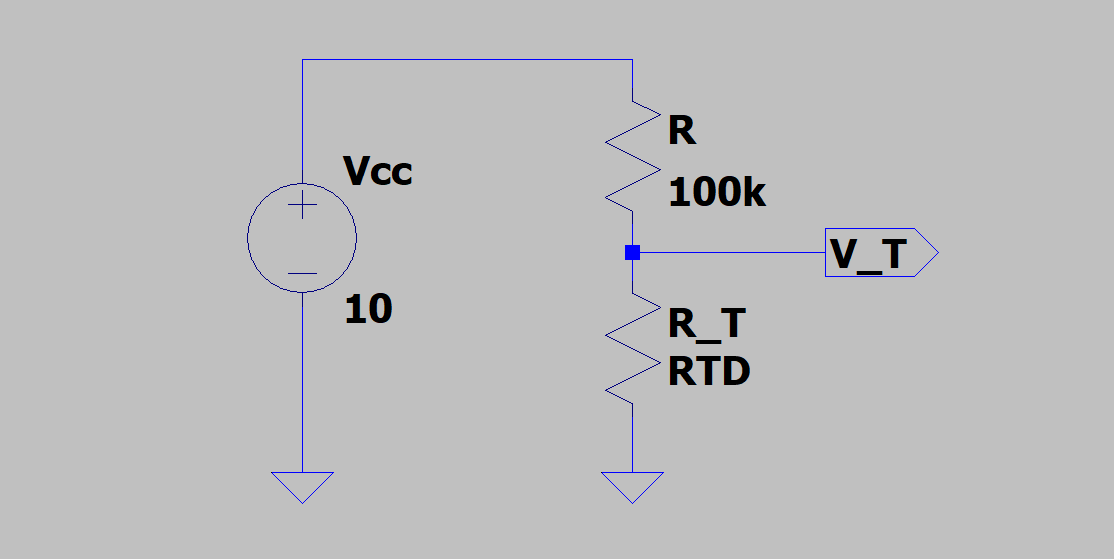
\includegraphics[width = \columnwidth]{images/circuito_div_tension.png}
	\caption{Circuito de medición (divisor de tensión) para el sensor de temperatura resistivo (RTD).}
    \label{fig:circuito_div_tension}
\end{figure}

A continuación se muestra el procedimiento utilizado para calcular el valor de R.

\begin{gather*}
    I = \frac{V_{CC}}{R_{eq}} \\
    \Longrightarrow 0.1 mA = \frac{10 V}{R_{eq}} \\
    \Longrightarrow R_{eq} = 100 k\Omega
\end{gather*}

\begin{gather*}
    R_{eq} = R + R_{T} \\
    \Longrightarrow R = R_{eq} - R_{T} \\
    \Longrightarrow R = 100 k\Omega - 100 \Omega \\
    \Longrightarrow R = 99 900 \Omega
\end{gather*}

Por conveniencia en la selección de componentes se decide utilizar un valor de $100 k\Omega$ para la resistencia R, ya que este es el valor más cercano al obtenido y que sigue mantiendo la corriente en el circuito menor a la corriente máxima permitida por el sensor.


\section{Tensiones de salida en el sensor de temperatura resistivo} 
A partir del circuito obtenido en la sección anterior, se utiliza la ecuación de divisor de tensión (Ecuacion \ref{eq:div_tension}) para calcular las tensiones de salida del sensor (Tabla \ref{tab:tensiones_salida}).

\begin{equation} \label{eq:div_tension}
    V_{T} = V_{CC}\frac{R_{T}}{R_{T}+R}
\end{equation}

\begin{table}[htb]
    \begin{center}
        \caption{Tensiones de salida para el RTD del circuito de medición de la Figura \ref{fig:circuito_div_tension}.}
        \label{tab:tensiones_salida}
        \begin{tabular}{c | c | c | c | c | c | c | c}
            \hline
            R ($\Omega$) & 100 & 108 & 119 & 127 & 131 & 134 & 138 \\
            \hline
            T ($^{\circ}C$) & 0 & 20 & 50 & 70 & 80 & 90 & 100  \\
            \hline
            $V_{T}$ (mV) & 9.99 & 10.78 & 11.86 & 12.68 & 13.08 & 13.38 & 13.78  \\
            \hline
        \end{tabular}
    \end{center}
\end{table}


\section{Acondicionamiento de la señal }
Se desea acondicionar los valores de tensión obtenidos (Tabla \ref{tab:tensiones_salida}) a un rango de 0 a 5V, manteniendo el rango de temperatura de $0^{\circ}C$ a $100^{\circ}C$. Esto porque los valores obtenidos del sensor son en el orden de los mV y al ser valores tan pequeños son fácilmente confundidos con el ruido, razón por la cual se desean amplificar y así tener una lectura más confiable y sencilla de ver.

\subsection{Acondicionamiento de la señal con un amplificador operacional}
\subsubsection{Obtención del circuito de medición acondicionado}

Para amplificar la señal se agrega un amplificador operacional no inversor (figura \ref{fig:op_amp}) al circuito de medición de la figura \ref{fig:circuito_div_tension}. Note que la tensión de salida del sensor es la misma que la entrada al acondicionador y se denota como $V_{T}$, y la tensión de salida del acondicionador se denota como $V_{OUT}$.

\begin{figure}[hbtp]
	\centering
	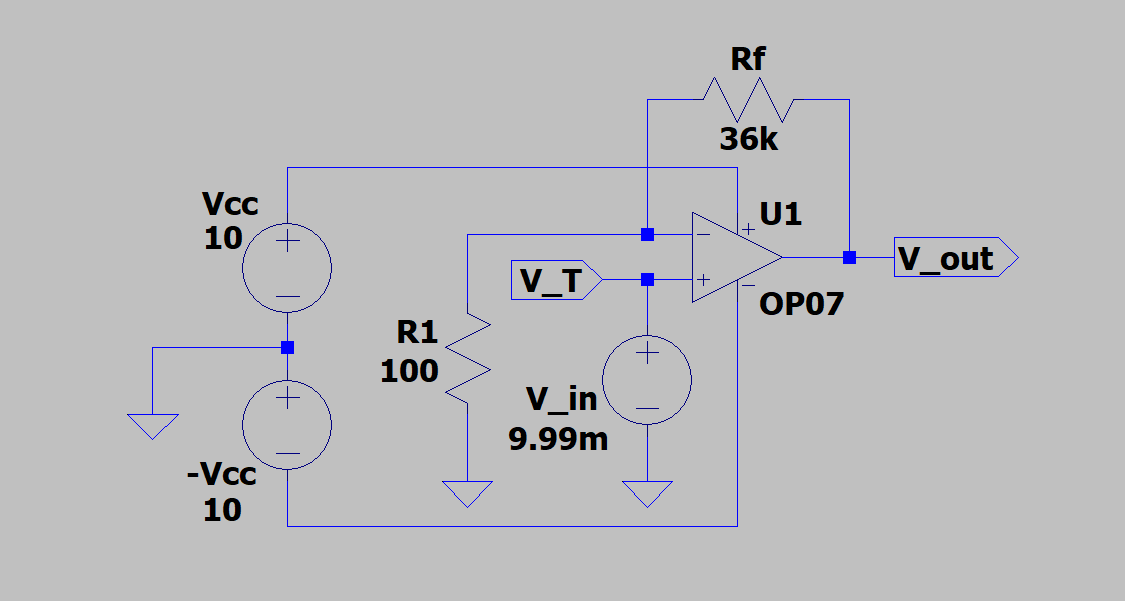
\includegraphics[width = \columnwidth]{images/op_amp.PNG}
	\caption{Etapa de acondicionamiento con un amplificador operacional en modo no inversor.}
    \label{fig:op_amp}
\end{figure}

El amplificador operacional utilizado posee la siguiente relación entre la tensión que recibe de entrada y la tensión de salida (ecuación \ref{eq:ecuacion_op_amp}).

\begin{equation}
    \label {eq:ecuacion_op_amp}
    V_{OUT} = V_{IN}(1+\frac{R_{f}}{R_{1}})
\end{equation}

El factor $(1+\frac{R_{f}}{R_{1}})$ corresponde a la ganancia de amplificador operacional y se elige de forma que las tensiones de salida de la tabla \ref{tab:tensiones_salida} se puedan amplificar al rango deseado (0V - 5V). Para esto, se calculan los valores de $R_{f}$ y $R_{1}$ a partir de las tensiones máximas, tanto la obtenida (13.78 mV) como la deseada (5 V).

\begin{gather*}
    5V = (1+\frac{R_{f}}{R_{1}})13.78mV \\
    \Longrightarrow (1+\frac{R_{f}}{R_{1}}) = \frac{5 V}{13.78 mV} \\
    \Longrightarrow \frac{R_{f}}{R_{1}} = 362.85-1 \\
    \Longrightarrow \frac{R_{f}}{R_{1}} = 361.85
\end{gather*}

Para aproximar el valor de ganancia requerido se proponen los siguientes valores para las resistencias: $R_{f}=36 k\Omega$ y $R_{1}=100 \Omega$. Obteniendo con estos una amplificación de 360 con respecto a la señal original.

Una vez obtenidala ganancia requerida, se calculan los valores de tensión de salida acondicionados al rango deseado con la ecuación \ref{eq:ecuacion_op_amp}. Estos se presentan en la tabla \ref{tab:tensiones_salida_acondicionados}.

\begin{table}[htb]
    \begin{center}
        \caption{Tensiones de salida acondicionadas a partir del circuito de la Figura \ref{fig:op_amp}.}
        \label{tab:tensiones_salida_acondicionados}
        \begin{tabular}{c | c | c | c | c | c | c | c}
            \hline
            R ($\Omega$) & 100 & 108 & 119 & 127 & 131 & 134 & 138 \\
            \hline
            T ($^{\circ}C$) & 0 & 20 & 50 & 70 & 80 & 90 & 100 \\
            \hline
            $V_{T}$ (mV) & 9.99 & 10.78 & 11.86 & 12.68 & 13.08 & 13.38 & 13.78 \\
            \hline
            $V_{OUT}$ (V) & 3.60 & 3.88 & 4.27 & 4.57 & 4.71 & 4.82 & 4.96 \\
            \hline
        \end{tabular}
    \end{center}
\end{table}

\subsubsection{Simluación en LTSpice}

Al simular el circuito de la figura \ref{fig:op_amp}, asignandole a la fuente $V_{IN}$ las tensiones de salida del sensor ($V_{T}$), se obtienen las siguientes tensiones acondicionadas (tabla \ref{tab:tensiones_salida_simuladas_op_amp}). El modelo del amplificador operacional utilizado corresponde al OP07 de Analog Devices.

\begin{table}[htb]
    \begin{center}
        \caption{Tensiones de salida simuladas para la etapa de acondicionamiento con un amp.op. (Figura \ref{fig:op_amp}.)}
        \label{tab:tensiones_salida_simuladas_op_amp}
        \begin{tabular}{c | c | c | c | c | c | c | c}
            \hline
            R ($\Omega$) & 100 & 108 & 119 & 127 & 131 & 134 & 138 \\
            \hline
            T ($^{\circ}C$) & 0 & 20 & 50 & 70 & 80 & 90 & 100 \\
            \hline
            $V_{T}$ (mV) & 9.99 & 10.78 & 11.86 & 12.68 & 13.08 & 13.38 & 13.78 \\
            \hline
            $V_{OUT}$ (V) & 3.53 & 3.81 & 4.20 & 4.49 & 4.63 & 4.73 & 4.88 \\
            \hline
        \end{tabular}
    \end{center}
\end{table}

\subsection{Acondicionamiento de la señal con un amplificador de instrumentación}

\subsubsection{Obtención del circuito de medición acondicionado}

Se utiliza un amplificador de instrumentación modelo LT1167 de Analog Devices. A partir de la hoja de datos se obtiene la siguiente relación entre la tensión de entrada recibida y la tensión de salida (ecuacion \ref{eq:ecuacion_op_amp_inst}).

\begin{equation} 
    \label {eq:ecuacion_op_amp_inst}
    V_{OUT} = V_{IN}(\frac{49.4k\Omega}{R_{G}}+1)
\end{equation}

Sabemos que la ganancia deseada es de $G=\frac{V_{OUT}}{V_{IN}}=361.85$. Despejando $R_{G}$ de la ecuación \ref{eq:ecuacion_op_amp_inst} obtenemos la ecuación \ref{eq:ecuacion_rg_inst}.

\begin{equation}
    \label {eq:ecuacion_rg_inst}
    R_{G} = \frac{49.4k\Omega}{G-1}
\end{equation}

Desarrollando,

\begin{gather*}
    R_{G} = \frac{49.4k\Omega}{361.85-1} \\
    R_{G} = 136.9 \Omega
\end{gather*}

Se elije utilizar $R_{G}=140$ por conveniencia en la selección de componentes. Una vez obtenido el valor de $R_{G}$ se define el circuito de la figura \ref{fig:op_amp_inst} para la etapa de acondicionamiento con amplificador de instrumentación.

\begin{figure}[hbtp]
	\centering
	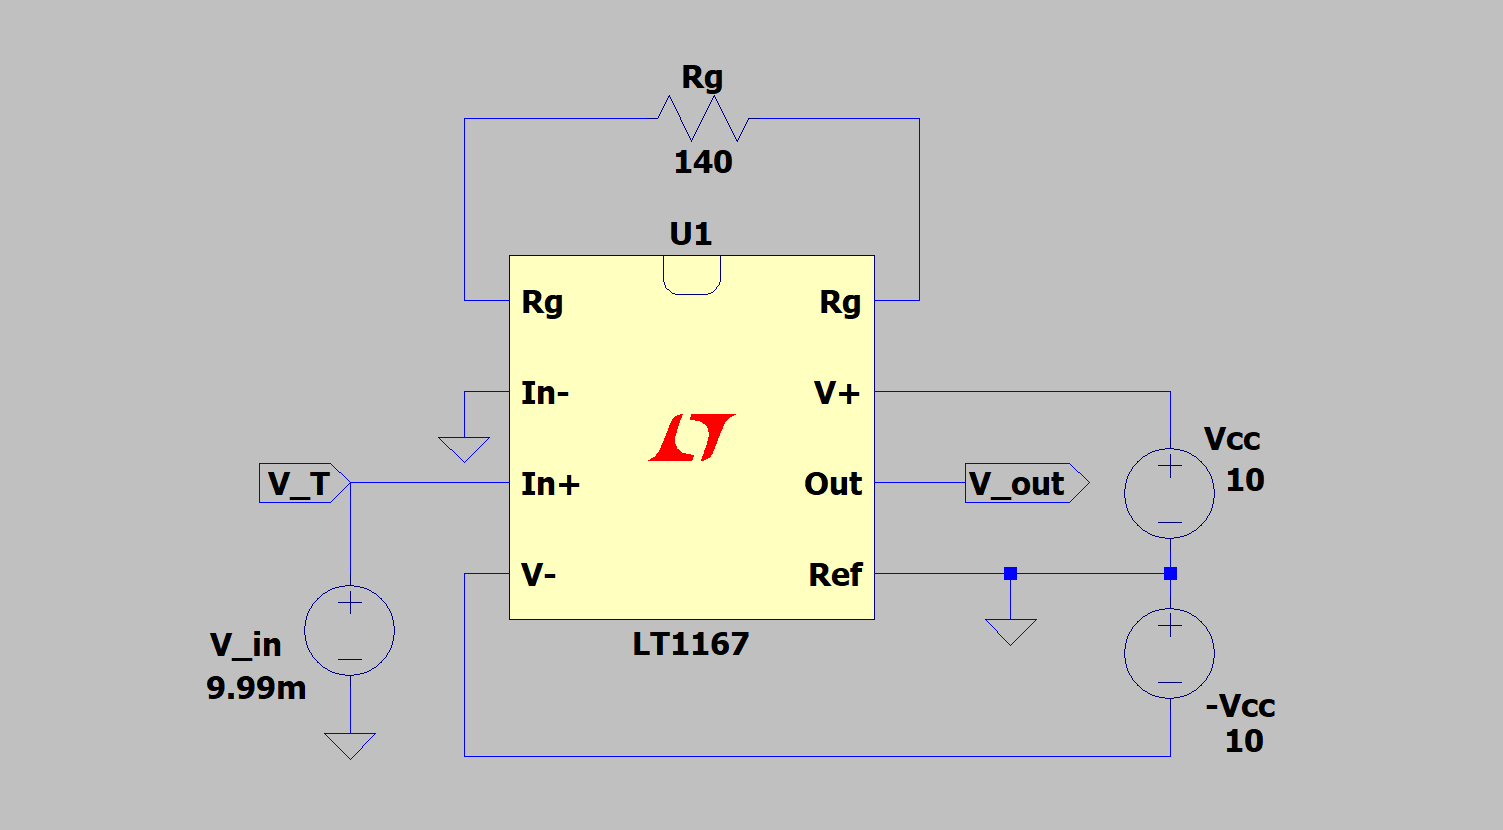
\includegraphics[width = \columnwidth]{images/op_amp_inst.PNG}
	\caption{Etapa de acondicionamiento con un amplificador operacional de instrumentación.}
    \label{fig:op_amp_inst}
\end{figure}


\subsubsection{Simluación en LTSpice}
Al simular el circuito de la figura \ref{fig:op_amp_inst}, asignandole a la fuente $V_{IN}$ las tensiones de salida del sensor ($V_{T}$), se obtienen las siguientes tensiones acondicionadas (tabla \ref{tab:tensiones_salida_simuladas_instr}).

\begin{table}[htb]
    \begin{center}
        \caption{Tensiones de salida simuladas para la etapa de acondicionamiento con un amp. de instrumentación (Figura \ref{fig:op_amp_inst}).}
        \label{tab:tensiones_salida_simuladas_instr}
        \begin{tabular}{c | c | c | c | c | c | c | c}
            \hline
            R ($\Omega$) & 100 & 108 & 119 & 127 & 131 & 134 & 138 \\
            \hline
            T ($^{\circ}C$) & 0 & 20 & 50 & 70 & 80 & 90 & 100 \\
            \hline
            $V_{T}$ (mV) & 9.99 & 10.78 & 11.86 & 12.68 & 13.08 & 13.38 & 13.78 \\
            \hline
            $V_{OUT}$ (V) & 3.61 & 3.89 & 4.28 & 4.58 & 4.72 & 4.83 & 4.97 \\
            \hline
        \end{tabular}
    \end{center}
\end{table}


%%%%%%%%%%%%%%%%%%%%%%%%%%%%%%%%%%%%%%%%%%%%%%%%%%%%%%%%%%

% trigger a \newpage just before the given reference
% number - used to balance the columns on the last page
% adjust value as needed - may need to be readjusted if
% the document is modified later
%\IEEEtriggeratref{8}
% The "triggered" command can be changed if desired:
%\IEEEtriggercmd{\enlargethispage{-5in}}

% references section

% can use a bibliography generated by BibTeX as a .bbl file
% BibTeX documentation can be easily obtained at:
% http://www.ctan.org/tex-archive/biblio/bibtex/contrib/doc/
% The IEEEtran BibTeX style support page is at:
% http://www.michaelshell.org/tex/ieeetran/bibtex/
%\bibliographystyle{IEEEtran}
% argument is your BibTeX string definitions and bibliography database(s)
%\bibliography{IEEEabrv,../bib/paper}
%
% <OR> manually copy in the resultant .bbl file
% set second argument of \begin to the number of references
% (used to reserve space for the reference number labels box)

%%%%%%%%%%%%%%%%%%%%%%%%%%%%%%%%%%%%%%%%%%%%%%%%%%
%\begin{thebibliography}{1}
%\bibitem{stat}
%Pakzad, S. N., \& Fenves, G. L. (2009). \emph{Statistical analysis of vibration modes of a suspension %bridge using spatially dense wireless sensor network}. Journal of structural engineering, 135(7), 863-872.
%\bibitem{stat1}
%Pakzad, S. N., Fenves, G. L., Kim, S., \& Culler, D. E. (2008).  \emph{Design and implementation of scalable wireless sensor network for structural monitoring}. Journal of Infrastructure Systems, 14(1), 89-101.
%\end{thebibliography}
%%%%%%%%%%%%%%%%%%%%%%%%%%%%%%%%%%%%%%%%%%%%%%%%%%

% biography section
% 
% If you have an EPS/PDF photo (graphicx package needed) extra braces are
% needed around the contents of the optional argument to biography to prevent
% the LaTeX parser from getting confused when it sees the complicated
% \includegraphics command within an optional argument. (You could create
% your own custom macro containing the \includegraphics command to make things
% simpler here.)
%\begin{IEEEbiography}[{\includegraphics[width=1in,height=1.25in,clip,keepaspectratio]{mshell}}]{Michael Shell}
% or if you just want to reserve a space for a photo:

%\begin{IEEEbiography}{Michael Shell}
%Biography text here.
%\end{IEEEbiography}

% if you will not have a photo at all:
%\begin{IEEEbiographynophoto}{John Doe}
%Biography text here.
%\end{IEEEbiographynophoto}

% insert where needed to balance the two columns on the last page with
% biographies
%\newpage

%\begin{IEEEbiographynophoto}{Jane Doe}
%Biography text here.
%\end{IEEEbiographynophoto}

% You can push biographies down or up by placing
% a \vfill before or after them. The appropriate
% use of \vfill depends on what kind of text is
% on the last page and whether or not the columns
% are being equalized.

%\vfill

% Can be used to pull up biographies so that the bottom of the last one
% is flush with the other column.
%\enlargethispage{-5in}



% that's all folks
\end{document}
